% !TEX root = ../midtermreport.tex
% !Mode:: "TeX:UTF-8"

\chapter{论文工作计划}
\label{chap:research_plan}

\section{论文研究目标}
\label{sect:research_goal}

% 介绍热带气旋
本论文主要研究一种常见的天气现象---热带气旋的模拟与仿真技术。
热带气旋(Tropical Cyclone,简称TC)
指的是一种快速旋转的风暴天气系统,有一个低气压中心和螺旋结构的云体,
同时伴随着强风、雷电、暴雨等现象,也被称作台风、飓风、热带风暴、气旋风暴、热带低压等。
一个成熟的热带气旋通常有完整的结构,其结构如图\ref{fig:tc_structure}所示,主要包括风眼,地面低压,暖心,中心密集云层区,风眼墙,螺旋雨带,外散环流等构成。
\begin{figure}[h!]
	\centering
	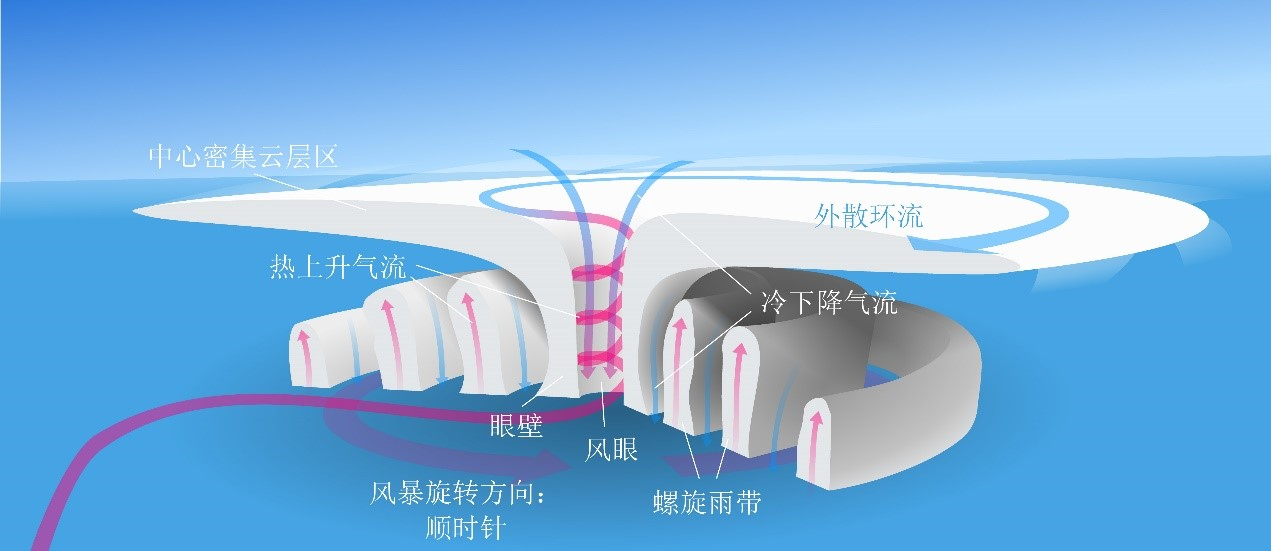
\includegraphics[width=400bp]{figure/tcstructure.jpg}
	\caption{热带气旋结构图}
	\label{fig:tc_structure}
\end{figure}

% 介绍研究意义
热带气旋的模拟和仿真技术一直是气象、海洋等领域演技研究的重点和难点,
而在计算机图形图像学领域,由于其独特的结构,热带气旋也是作为一个重要的研究内容。
其中主要包括研究热带气旋的可视化效果,云的真实感绘制技术,以及热带气旋的模拟技术。
同时能够较真实的模拟热带气旋的运动以及真实的展现其结构,
对气象研究、海洋研究、气象预测等具有极其重要的意义。

% 研究现状
在计算机图形图形领域,对热带气旋方面的的研究主要集中在对云的建模和仿真。
随着虚拟场景渲染技术的发展,云的模拟表现也成为计算机图形学和虚拟现实技术中的热门课题。
云的真实感模拟不仅能有效提高场景逼真度,更能传达丰富的气象信息。
云作为一种常见的自然现象,由于其形状千变万化,形成、发展和消散的过程又极其复杂,
且具有水汽粒子的半透明特征。
能够实现即满足气象学应用,同时实现逼真展现的云场景模拟是一项很艰巨的任务。

早期在图形图像学领域云建模大体分为两类,
即基于过程的云建模和基于物理的云建模。
前者侧重于利用噪声、纹理或者交互式的手段对云进行建模,通常需要经历繁琐的参数调整;
后者则通过求解简化的NS方程,模拟云生成的物理过程,
这种方法耗时大,且不能有效生成预期形状的云。

基于数据驱动的云建模,在一定程度上能够克服之前建模方法的缺点,
且由于其建模过程中参考了真实数据,
能够在一定程度上反映数据信息、表达气象属性,因此具有很强的应用意义,逐渐成为研究的热点。
通过研究和分析云的相关数据(自然图像、观测数据、数值模拟数据、卫星云图等),
进一步从数据中发掘能够指导云建模的信息,
构建逼真的三维云场,同时与真实数据在形状、气象信息、规模上具有一定相关性。
相应的成果可以为天气数值预测、军事仿真、卫星气象等领域提供可视化工具和环境。

% 本论文的意义
基于时变气象数据的热带气旋的仿真技术,相比于传统的图形图像学建模方法,
由于使用的是数值模拟数据(Weather Research and Forecasting Model,简称WRF)进行建模,
模型本身就具有真实性,同时通过时序数据的矫正,使得仿真的数据气象学的意义,
符合气象学用户对数据准确性的要求;
同时又在时域内使用简单NS方程模拟云的运动过程,使得模拟速度能够达到实时应用的需求。

综述所述,热带气旋仿真技术具重要的研究意义以及广阔的应用前景,
但是现有方法建模过程难以实现及满足气象需求,同时满足逼真展现的应用。
因此,本文提出的仿真方法具有重要的意义。

% 研究目标
本论文的研究目标:针对热带气旋这一种复杂的天气系统,
设计并实现一个热带气旋的动态仿真模拟算法。 
该算法使用气象数据做初始状态,同时以长时间跨度的时变气象数据为输入,
使用基于位置的流体仿真(position based Fluids,简称PBF)方法,利用GPU加速计算云的仿真,
输出指定时间跨度的粒子数据,在保留更多细节的同时,保证仿真过度自然流畅。

在此基础上,结合基于粒子的云建模方法和
基于粒子系统的LOD(Level of Detail)层级结构的绘制方法,
形成包括建模、仿真、绘制的热带气旋动态仿真系统。

\section{论文主要研究内容}

本论文的主要研究内容包括:
提取WRF数据中的云相关建模参量建立云的粒子模型,
根据使用PBF仿真技术模拟云的运动过程,
根据WRF数据中的每一帧数据,校正PBF流体仿真产生的误差,
最后基于粒子系统的LOD层级结构,使用多散射模型的绘制方法绘制具有真实感的云。
流程图如图\ref{fig:research_contents}

本论文主要研究的内容如图\ref{fig:research_contents}所示,该图给出了整个系统的模块划分和模块之间的输入输出关系。具体内容阐述如下:
\begin{figure}[h!]
	\centering
	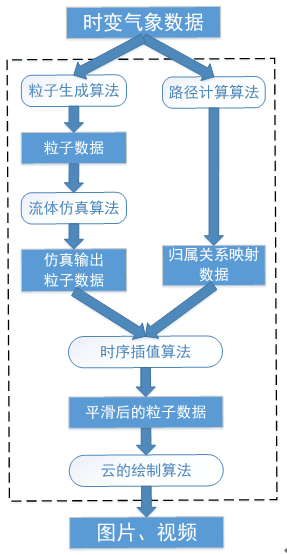
\includegraphics[width = 150bp]{figure/researchContemts.png}
	\caption{基于时变气象数据的热带气旋动态仿真技术研究流程图}
	\label{fig:research_contents}
\end{figure}



